\documentclass{epsrc}


%----These packages are only needed for drafts-----%
\usepackage{lipsum} % used for dummy text
\usepackage[colorinlistoftodos,prependcaption,textsize=tiny]{todonotes}%to do list and comments
\usepackage{soul}%highlighting etc
%--------------------------------------%


%I use these routinely but may not be needed
\usepackage{chemstyle}
\usepackage[version=3]{mhchem}
\usepackage{graphicx}
\usepackage{amsmath}
\usepackage{amsfonts}
\usepackage{pgfgantt}
\usepackage{pdflscape}

%required for wrapping text around figures
\usepackage{wrapfig}

%set up different captions
\usepackage{caption}
\captionsetup[figure]{labelfont={it,bf},textfont=it}

%set up two bibliographies for parts 1 and 2
\usepackage[resetlabels]{multibib}
\newcites{A,B}{References,%
References}

\usepackage[british]{babel}

%%%Fancy header settings. Remove draft parts for final
\usepackage{fancyhdr}
\setlength{\headheight}{20pt}
\pagestyle{fancy}
\lhead[COMP5840M Data Mining and Text Analytics]%
{COMP5840M Data Mining and Text Analytics}
\rhead[School of Computing]%
{School of Computing}
\cfoot[\thepage]{\thepage}

\begin{document}

\begin{titlepage}

\newcommand{\HRule}{\rule{\linewidth}{0.5mm}} % Defines a new command for the horizontal lines, change thickness here

\center % Center everything on the page
 
%----------------------------------------------------------------------------------------
%	HEADING SECTIONS
%----------------------------------------------------------------------------------------

\textsc{\LARGE University Of Leeds}\\[1cm] % Name of your university/college
\textsc{\Large School of Computing}\\[0.5cm] % Major heading such as course name
\textsc{\large COMP5840M - Data Mining and Text Analytics}\\[0.5cm] % Minor heading such as course title

%----------------------------------------------------------------------------------------
%	TITLE SECTION
%----------------------------------------------------------------------------------------

\HRule \\[0.5cm]
{ \huge \bfseries Voice - Based Route Navigator Using Automatic Speech Recognition (ASR) and Natural Language Processing (NLP)}\\[0.4cm] % Title of your document
\HRule \\[2cm]
 
%----------------------------------------------------------------------------------------
%	AUTHOR SECTION
%----------------------------------------------------------------------------------------

% If you don't want a supervisor, uncomment the two lines below and remove the section above
\Large \emph{Team Name:} \textsc{Data Warriors}\\[2cm] % Your name
\Large \emph{Team Members:} \\
\emph{Katuru Venkata Sai [mm22kvs]}\\
\emph{Komal Katta [sc22k2ck]}\\
\emph{Mani Mandepudi [mm22mkm]}\\
\emph{Mounica Ghanta [mm22m2g]}\\
\emph{Nilesh Kumar [mm22nk]}\\
\emph{Makarand Batchu [mm22mpb]}\\[2cm]

%----------------------------------------------------------------------------------------
%	DATE SECTION
%----------------------------------------------------------------------------------------
{\large \emph{Date:} \today}\\[1cm] % Date, change the \today to a set date if you want to be precise

\vfill % Fill the rest of the page with whitespace

\end{titlepage}
\newpage

\part{Background}


%This is a sample text to check the reference to my base reference %paper using bibliographyA\citeA{8629859}

%This is a sample text to check the reference to my base reference paper using bibliographyB\citeB{8629859}

%\lipsum[1-14]
%\bibliographystyleA{angew}
%\bibliographyA{refs}
%\bibliographyB{refs}
\vspace{5pt}

Many businesses, particularly transportation systems, have experienced tremendous development as a result of recent technological advancements. Global navigation satellite systems (GNSS) like GPS, GLONASS, and Galileo have revolutionised how people move and travel. Interest in human-computer interaction research has concurrently risen, particularly in the application of voice and speech. Through the use of automatic speech recognition (ASR) and natural language processing (NLP) technology, this research seeks to combine GNSS and human-computer interaction.
\vspace{5pt}

In existing navigation systems, users must specify the starting location and ending location of their journey as user inputs to the system, and the system then returns all possible routes between those two locations. However, if the user cannot specify the exact location, they will not be able to use those systems. Although there might not be a name for the destination location on the map or the user might not be able to pinpoint the destination location, they might know the directions to it. Therefore, if a navigation system could map the route when the user explains the directions to their destination, the existing navigation system's limitation would be overcome. 
\vspace{5pt}

Taking inspiration from a paper on road navigation system\cite{8629859} and building on top of it, we present a mobile road navigation system that will detect and modify audio input from the user using ASR, followed by NLP to provide a route in the map using Google Map API. The system will then compare the user-preferred route against a Google Maps route in terms of time to destination, traffic, and other such criteria, and provide the user with the choice to choose between the two. 
\vspace{5pt}

The system will be designed to be able to provide instructions in languages other than English through machine translation, broadening its appeal to a global target market. To provide hands-free operation and smooth operation, the device may be built to respond to a programmable wake word for voice activation.
\vspace{5pt}

The proposed theory is supported by earlier and current studies carried out in the UK and internationally. ASR system development has long been a top focus, and current developments in deep learning and neural networks have greatly advanced this field. The Google ASR system, Amazon’s Alexa and Apple's Siri are some examples of ASR technology products that have incorporated themselves into our daily lives.
\vspace{5pt}

In the United Kingdom, universities such as the University of Cambridge, the University of Edinburgh, and Imperial College London, among others, have conducted ASR and NLP research. These esteemed universities have made major contributions to the subject, including the development of novel algorithms and models. Internationally, initiatives like the European Union's Horizon 2020 programme, which funded a variety of studies related to speech and language processing, have supported the advancement of ASR and NLP technologies. Organisations such as the National Science Foundation and the Defence Advanced Research Projects Agency (DARPA) in the United States has funded research in this sector as well.
\vspace{5pt}

The proposed road navigation system intends to combine current breakthroughs in ASR and NLP, such as machine translation and wake word detection, into a unified solution. By combining cutting-edge research and real-world applications, this project aims to address the difficulties of multilingual communication and hands-free interaction in the context of road navigation. Finally, this significant advancement has the potential to transform how people interact with navigation systems, making travel safer, more efficient, and more inclusive for users all across the world. 

\part{Contribution to knowledge}
\vspace{5pt}

The mobile road navigation system introduced contributes to the fields of speech recognition, natural language processing, navigation technology and mobile computing.. The system provides an efficient way for converting natural language directions into a form that a machine may utilise to provide turn-by-turn directions on a map by integrating automated speech recognition (ASR) and natural language processing (NLP). 
\vspace{5pt}

According to the past literature evaluation and analysis of the features in most navigation systems, it is clear that most present navigation systems do not enable dynamic route mapping based on user-defined directions delivered as voice commands. As a result, in our suggested system, we include the capability of mapping the instructions provided by the user in voice commands.
\vspace{5pt}

This not only improves usability and practicality, but it also removes a significant hurdle to mobile navigation system adoption: the requirement for users to manually enter their location. Users can interact with the system using natural language commands, which eliminates the need for visual input and reduces the cognitive load required to navigate while driving.
\vspace{5pt}

Additionally, this system can contribute to the reduction of distracted driving, a major cause of road accidents worldwide. By enabling drivers to interact with the system using voice commands, they can keep their eyes on the road and hands on the wheel, minimizing the risk of accidents caused by distracted driving.
\vspace{5pt}

Machine translation would increase the system's attractiveness in the worldwide market. The ability of the system to deliver directions in languages other than English broadens its appeal and makes it an appealing alternative to a wider audience. This helps the field of multilingual computing, which is focused with creating systems that can handle different languages. The response of the system to a programmable wake word for voice activation relates to the field of human-computer interaction, which is concerned with building systems that are intuitive and simple to use.
\vspace{5pt}

Furthermore, the development of this system can lead to improvements in the efficiency and accuracy of road navigation systems. By utilizing ASR and NLP technology, the system can accurately understand and interpret user input, even in noisy or challenging environments, resulting in more precise navigation instructions and improved user satisfaction.
\vspace{5pt}

The proposed system contributes to several fields of study, including speech recognition, natural language processing, transportation engineering, multilingual computing, and human-computer interaction. The system's ability to provide efficient, hands-free, and personalized navigation directions has the potential to improve the travel experience of millions of people worldwide.

\part{Importance}
\vspace{5pt}

The proposed system can considerably boost the current and future growth of the navigation and transportation industry.  This is especially true in developing countries where not every location is marked on a map and users may struggle to find a location on the navigation system to which they are already familiar with the path. Additionally, it would be a great mobile application for users who are less tech-savvy and prefer to talk rather than use a mobile phone to navigate. Therefore, it can provide a more accessible and user-friendly option for both individuals and businesses due to its innovative take on navigation. 
\vspace{5pt}

It can drastically decrease the navigation costs for companies that majorly depend on effective transportation systems, which has a positive impact on economic growth. Businesses can streamline delivery routes, and reduce transportation-related time and expenses by using real-time traffic reports. Additionally, providing a more personalized experience that addresses specific requirements can help businesses strengthen their ties with their clients.
\vspace{5pt}

Emerging industries such as the autonomous vehicle industry can also benefit from the proposed system. The use of NLP, ASR, and Google Map API may deliver more reliable and accurate navigation that can facilitate this growth as they become more mainstream.
\vspace{5pt}

Additionally, the system can address key societal challenges such as safety and accessibility. The use of voice commands supported  in multiple languages and natural language processing can make it more accessible for those with disabilities, promising a less complicated navigation experience. And the focus on offering a safer experience of driving may help lower the rate of accidents brought on by distracted driving, making transportation more safe.
\vspace{5pt}

\part{Research Hypothesis and Objectives}
\vspace{5pt}

Our hypothesis is that developing a voice-based navigation system will offer an efficient way to translate natural language directions into a machine-understandable format and in turn bridge the gap between human and machine.
\vspace{5pt}

Considering how much popularity voice assistants have gained in our lives, voice-based navigation systems hold potential to revolutionize the way we interact with machines. The proposed system, is a novel approach to develop a user-centric road navigation mobile application that can efficiently translate natural language directions to a machine-understandable format. This system's scientific ambition is to improve human-machine interaction and make navigation more accessible and intuitive for users.
\vspace{5pt}

The measurable objectives against which the outputs, outcomes, and impacts of the work will be assessed are:
\vspace{5pt}
\begin{enumerate}
    \item Investigate the current state-of-the-art methodologies in ASR and NLP relevant to mobile road navigation systems, and identify key features and requirements for an efficient voice-based system.
    \item Develop an Automatic Speech Recognizer (ASR) to convert audio streams into text with high accuracy.
    \item Utilize the suitable frameworks to perform Natural Language Processing (NLP) on the text to retrieve navigation-associated information, including street names, landmarks, point of interests, junctions, etc.
    \item Process the route using Google Map API, including the user's preferred route, turn-by-turn directions, and mapping the route in an interactive interface.
    \item Design an intuitive user interface that supports hands-free operation and enables users to speak normally and ask for directions using everyday language.
    \item Assess the system's accuracy and efficiency by conducting user studies and evaluating natural language translation and route customization.
    \item Address any limitations or issues identified during the evaluation phase, and improve the accuracy and efficiency of the ASR and NLP components.
    \item Share the research findings and contribute to the progress of mobile road navigation systems, as well as evaluate the system's potential to revolutionise the human-machine interface for navigation systems .
\end{enumerate}
\vspace{5pt}

The integration of Automatic Speech Recognition (ASR) and Natural Language Processing (NLP) in road navigation systems will not only enhance user satisfaction and reduce journey time but also have a profound impact on various aspects of the driving experience. By providing more effective, accurate, and user-friendly navigation systems, ASR and NLP technologies can contribute to several additional benefits:
\vspace{5pt}
\begin{enumerate}
    \item \textbf{Increased Road Safety:} By enabling hands-free operation and minimizing distractions, the voice-based navigation system can help drivers maintain their focus on the road, thus reducing the risk of accidents.
    \item \textbf{Inclusion of Diverse User Groups:} The system's ability to understand and process everyday language (supporting languages other than English) will make it more accessible to users with varying levels of technical proficiency, language skills, and even those with certain disabilities, such as vision impairments.
    \item \textbf{Eco-friendly Route Planning:} By providing more accurate and efficient route suggestions, the system can help reduce fuel consumption and emissions, contributing to a more sustainable and environmentally-friendly transportation ecosystem.
\end{enumerate}
\vspace{5pt}

By exploring these additional benefits, the research on ASR and NLP-based road navigation systems can help create a more comprehensive understanding of the potential impact of such technologies on the future of transportation and human-machine interaction.

\part{Programme and Methodology}
\vspace{5pt}

\section{Business Understanding}
\vspace{5pt}

The problem statement for the proposed system is that existing road navigation systems have a limitation that they require users to input the exact starting and ending points of their journey and do not provide dynamic route mapping upon the user's customized preferred route given as voice commands. If the user is unable to specify the exact destination, they may not be able to use the navigation system effectively. But, users may know the route directions to their desired destination. Therefore, the proposed system aims to address this limitation by allowing users to give route directions in natural language (might be English or any of the other supported languages), which will be processed using automatic speech recognition and natural language processing to map the identified route for the user-defined endpoint. This proposed system was inspired by an existing paper\cite{8629859} and has been enhanced with new features to make it more user-friendly and accessible to a wider audience.
\vspace{5pt}

%The suggested system's main objective is to overcome the limitation of existing road navigation systems and to provide dynamic route mapping based on the user's customised preferred route delivered via voice commands. Additionally, this feature is supported by allowing users to provide voice commands in languages other than English. Furthermore, we want to make the proposed system more accessible to people who are less tech-savvy by including a wake word feature that commences recognising voice inputs when the user says a wake word. In addition to the above listed features, the proposed system intends to present the user with an option between the user-preferred path and an optimised path provided by Google Maps.
%\vspace{5pt}

%The development of a natural language-based navigation system can be a technically demanding task that involves advanced algorithms and software architectures. The accuracy of ASR and NLP models is crucial in designing a system that can recognise and process natural language user directions. Another technological aspect that requires close attention is the integration of various components with other technologies such as Map APIs, mobile operating systems, and other navigation systems. 
\vspace{5pt}

\section{Data Understanding}
\vspace{5pt}

To train a wake word detection algorithm, we must gather and label a dataset of audio recordings including samples of the wake word being pronounced in various settings and by various speakers. The dataset should consist of a wide range of voices, accents, and dialects that are typical of the user community for which the wake word detection algorithm is designed. This will help to ensure that the model recognises the wake word correctly in a range of real-world settings. The audio recordings should be labelled with timestamps indicating the beginning and ending of the wake word, as well as any background noise that may be present. This labelling will be used to train the model to detect and discriminate the wake word from other speech and noise.
\vspace{5pt}

The system would require the user to provide audio input in the form of spoken directions to their location for the language and acoustic model which is part of the ASR component. The recognition accuracy varies due to differences in pronunciation, speaker, and style of speech. Maximum-A-Posteriori (MAP) adaptation will be used on the acoustic model to increase accuracy. Recorded audio data containing navigation voice commands is required for this method. Furthermore, in order to achieve high accuracy in the system, the training process for the NLP model requires a large training data set for identifying different routes.
\vspace{5pt}

\section{Data Preparation}
\vspace{5pt}

Automatic speech recognition relies heavily on audio preparation. The goal of audio preprocessing is to prepare the raw audio signal for further processing by employing techniques that increase signal quality. We anticipate that the user may use the application while driving, which may result in background noise that makes it difficult for the app to effectively recognise speech. To optimise the application's speed, we are using audio preprocessing techniques like filtering, normalisation, compression, and equalization to reduce noise in the audio signal, resulting in increased audio clarity.
\vspace{5pt}

The ASR component's output will be used as input for the natural language processing component of the project architecture, but before passing the data, text preparation techniques will be used. Text preprocessing is a crucial stage in natural language and text analytics modeling since it involves converting raw text data into a more suitable format for analysis and modeling. This approach employs techniques including tokenisation, stemming, stop-word deletion, and normalisation. 
%Tokenisation is a process that involves breaking up a piece of text into smaller units called tokens. These tokens could be words, phrases, or even individual characters, depending on the specific use case. Stemming is a process that involves reducing words to their base or root form. Stemming is used to normalise words so that different variations of a word can be treated as the same word, which can improve the accuracy of some NLP tasks. Stop-word deletion is a technique used to remove common words, also known as stop words, from a piece of text before further processing. Stop words are words that occur frequently in a language and do not carry significant meaning, such as "the," "a," "an," "and," "in," "of," and "to.". Normalisation refers to the process of converting text into a standard or canonical form, which makes it easier to compare and analyze text data. The goal of normalisation is to reduce the complexity of text by removing noise and inconsistencies that can hinder NLP tasks.
\vspace{5pt}

\section{Modelling}

\begin{figure}[hbtp]
    \centering
    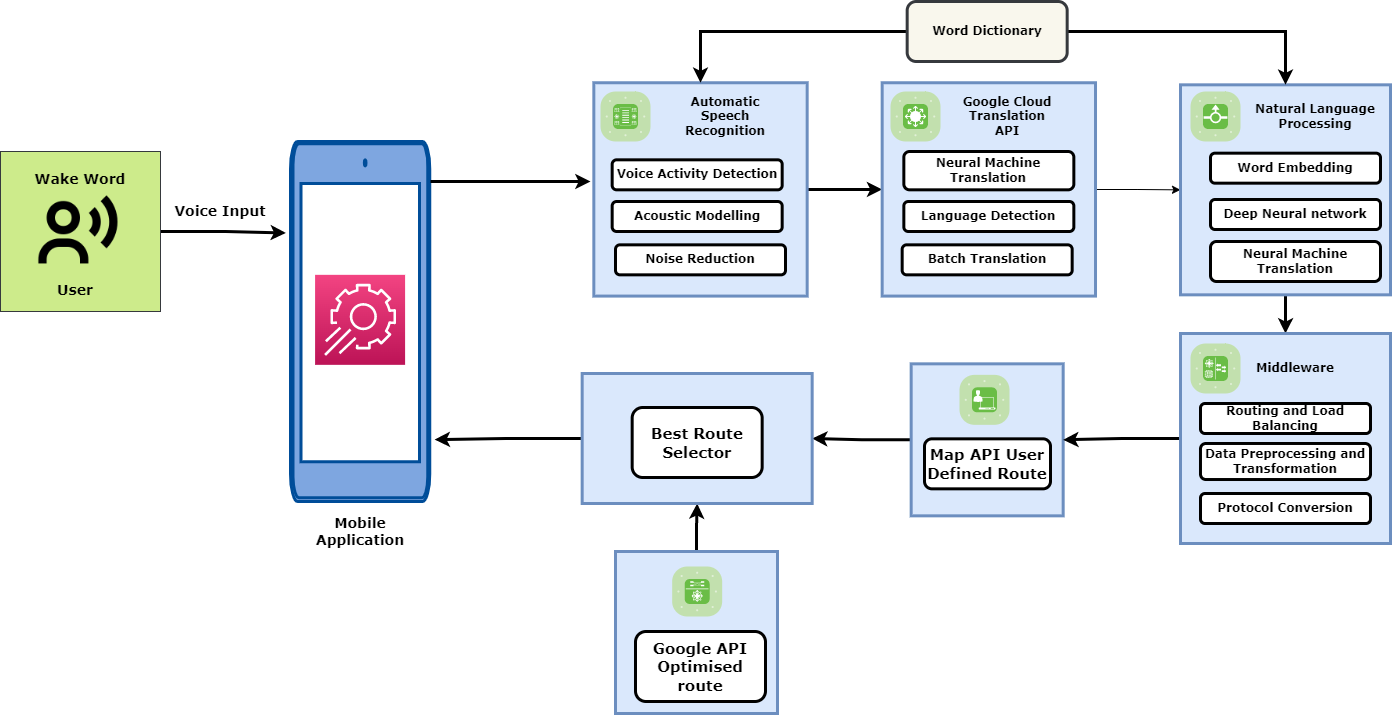
\includegraphics[width=17cm]{archi (1).png}
    \caption{Proposed System Design}
    \label{fig:Architecture}
\end{figure}
\vspace{5pt}

The modelling of a road navigation system using automatic speech recognition (ASR) and natural language processing (NLP) will be covered in this part. The technology aims to give consumers a smooth and user-friendly experience when they utilise voice input to get directions and navigation tips. As shown in \ref{fig:Architecture} ASR, Google Cloud Translation API, NLP, and Middleware make up the architecture's four key building blocks. Each component's characteristics and functions will be briefly described, along with how they work together to produce the desired results.
\vspace{5pt}

\subsection{Automatic Speech Recognition (ASR)}
The ASR component is responsible for transcribing the user's voice input into text. This process involves three main features:
\begin{enumerate}
    \item {\em Voice Activity Detection (VAD):} VAD is used to identify when a user starts and stops speaking.\cite{7995777}
    \item {\em Acoustic Modelling:} This feature aims to represent the relationship between speech sounds and their corresponding phonemes. It helps the system to recognize different accents and dialects.\cite{7995777}
    \item {\em Noise reduction:} This feature works to minimize the impact of background noise on the transcription process, ensuring that the voice input is clear and accurate.
\end{enumerate}
\vspace{5pt}

\subsection{Google Cloud Translation API}
The Google Cloud Translation API is utilized to translate the transcribed text (if required) and supports language detection and batch translation. The main features include:
\begin{enumerate}
    \item {\em Neural Machine Translation (NMT):} NMT models are used for translating text with high accuracy and fluency, making the translation process more efficient.
    \item {\em Language detection:} The API can automatically detect the input language, removing the need for users to specify their language manually.
    \item {\em Batch Translation:} This feature enables the system to process multiple translations simultaneously, which improves the overall performance and reduces processing time.
\end{enumerate}
\vspace{5pt}

\subsection{Natural Language Processing (NLP)}
The NLP component is responsible for extracting meaningful information from the transcribed text and translating it into navigation instructions. Key features include:
\begin{enumerate}
    \item {\em Word embedding:} This technique is used to convert words into numerical vectors, allowing the system to identify relationships between words and understand their contextual meaning.\cite{7995777}
    \item {\em Multi-word expressions:} The system can recognize and process compound words or phrases, enabling it to understand complex navigation requests accurately.
    \item {\em Deep neural networks (DNN) and Neural Machine Translation (NMT):} DNNs and NMT models are used to process and interpret the input text, ensuring accurate and contextually relevant translations and instructions.\cite{7995777}
\end{enumerate}
\vspace{5pt}


\subsection{Middleware}
The Middleware component is responsible for managing the communication between the different components of the system. Key features include:
\begin{enumerate}
    \item {\em Routing and Load Balancing:} This feature ensures that requests are distributed evenly across the system's resources, optimizing performance and reducing latency.
    \item {\em Data Pre-processing and Transformation:} The Middleware component preprocesses the input data to ensure it is in a format suitable for the other components.
    \item {\em Protocol conversion:} The Middleware component handles the conversion of protocols between the various components, ensuring smooth communication, integration and data exchange.
\end{enumerate}
\vspace{5pt}


\subsection{System Workflow}
The navigation system operates as follows:
\begin{enumerate}
    \item The user provides a voice input containing their turn-by-turn navigation directions.
    \item The ASR component transcribes the voice input into text.
    \item If the language is not English, the Google Cloud Translation API translates the transcribed text into the English language.
    \item The NLP component processes the text, extracting relevant information and generating navigation instructions.
    \item The Middleware component routes the navigation instructions to the appropriate services (e.g., Google Maps) and retrieves the user defined route.
    \item The Google Map AI will provide an optimized route, and the navigation system will display both the user-defined route and the optimal route as options. This allows the user to choose the best route.
\end{enumerate}
By leveraging the features and capabilities of each component, the proposed road navigation system aims to offers a seamless, user-friendly experience that allows users to effortlessly obtain accurate and contextually relevant directions through natural language voice input, enhancing their overall navigation experience and promoting safer and more efficient journeys.
\vspace{5pt}

\section{Evaluation}
\vspace{5pt}

To assess the performance and effectiveness of the proposed road navigation system, we will employ a multi-faceted evaluation approach, focusing on the following key aspects:

\begin{enumerate}
    \item {\em Accuracy:} The accuracy of the system will be evaluated by comparing the generated navigation instructions with the actual directions required to reach the destination. This includes assessing the quality of ASR transcription, translation, and NLP-generated instructions. A high accuracy rate would indicate that the system is capable of providing reliable directions.
    \item {\em Response Time:} The response time is a crucial aspect of the user experience. We will measure the time taken by the system to process user input and present the optimal route suggestions. A low response time would demonstrate the system's efficiency and its ability to handle real-time navigation requests effectively.
    \item {\em User Satisfaction:} A survey will be distributed to users to get input on their experience with the system. The questions will be designed to assess the simplicity of use, the quality of the guidance offered, and overall satisfaction with the system. High user satisfaction levels suggest that the system satisfies the requirements and expectations of its users.
\end{enumerate}
\vspace{5pt}

 The evaluation results will be analyzed to identify areas of improvement and potential optimizations. By addressing these areas, we aim to enhance the performance and user experience of the proposed road navigation system, making it a reliable and efficient tool for voice-based navigation assistance.
 \vspace{5pt}

\section{Deployment}
\vspace{5pt}

We will deploy the road navigation system as a mobile app using cloud technologies like AWS, Azure or GCP and Python, ensuring flexibility and scalability. Key steps include utilizing cloud platforms for infrastructure, adopting containerization technologies, implementing a CI/CD pipelines for version control, developing a cross-platform app, and employing cloud-based monitoring tools. This approach delivers a user-friendly, accessible mobile app that meets users' needs and can be efficiently maintained and improved over time.
\vspace{5pt}

\newpage

\part{Work-Plan Diagram}
\vspace{30pt}


\begin{figure}[hbtp]
    \centering
    \rotatebox{270}{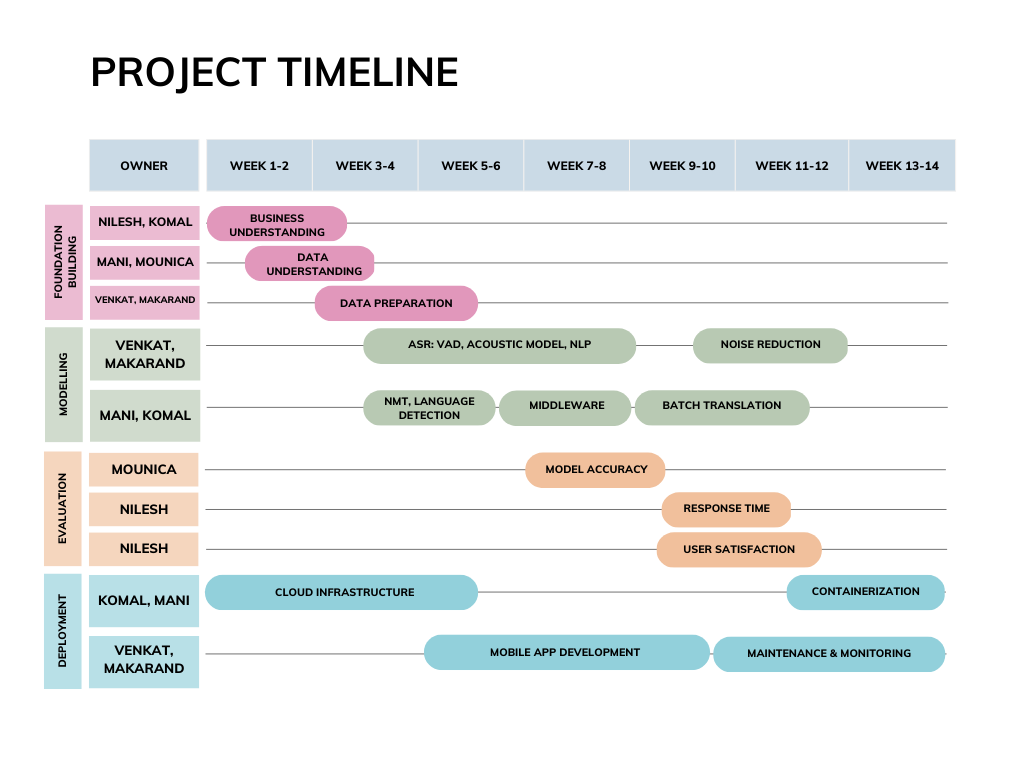
\includegraphics[width = 20cm]{Pastel Aesthetic departments Professional Gantt Graph (3).png}}
\end{figure}

\vspace{5pt}

\newpage

\part{Appendix}
\vspace{5pt}

In our research proposal, we utilized three powerful tools: \textbf{ChatGPT, Grammarly, and Google Scholar}. 
\vspace{5pt}

\section{Google Scholar}
\vspace{5pt}

\begin{figure}[hbtp]
    \centering
    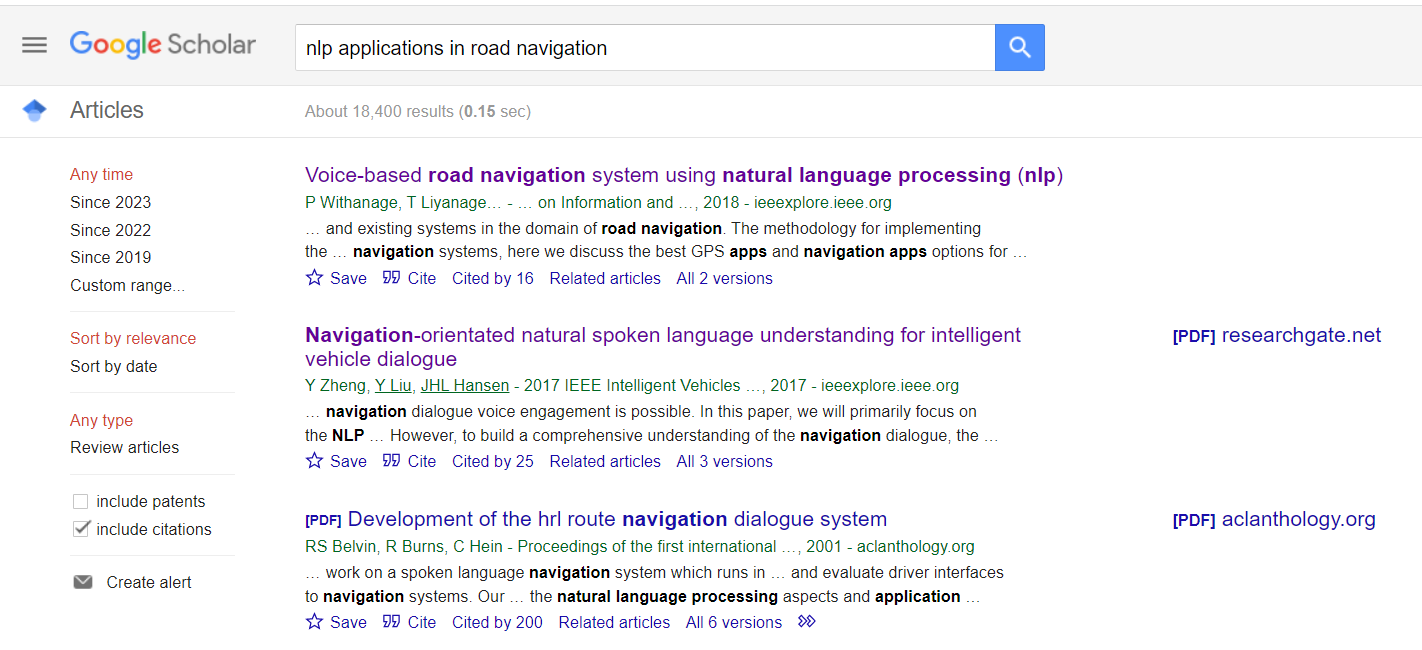
\includegraphics[width = 13.5cm]{google scholar.png}
    \caption{Google Scholar was used to perform research on our topic using published papers}
    \label{fig:GScholar}
\end{figure}
\vspace{5pt}

As seen in \ref{fig:GScholar}, we turned to Google Scholar for extensive research on our topic. With its vast database of academic articles, books, and conference papers, we were able to find relevant and up-to-date information to support our proposal.
\vspace{5pt}

\section{ChatGPT}
\vspace{5pt}

ChatGPT offered valuable insights and suggestions for our research topic. Its human-like text generation and understanding capabilities helped us refine our ideas and present them effectively.
\vspace{5pt}

\begin{figure}[hbtp]
    \centering
    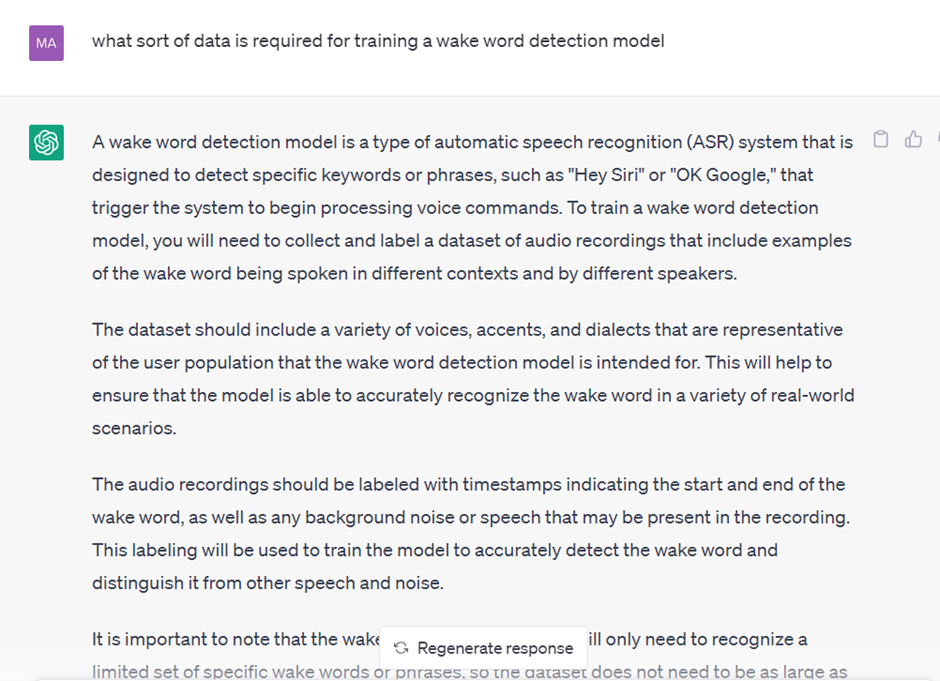
\includegraphics[width = 13.5cm]{WakeWord.png}
    \caption{ChatGPT prompt and response to acquire more information about data needed for the wake word model}
    \label{fig:wakeword}
\end{figure}
\vspace{5pt}

As seen in \ref{fig:wakeword}, for the data understanding phase of our methodology, we utilized ChatGPT to assist us in identifying the type of data that would be required to effectively train our wake word detection model. By leveraging this tool, we were able to gain valuable insights into the characteristics of the data needed for our project.
\vspace{5pt}

\begin{figure}[hbtp]
    \centering
    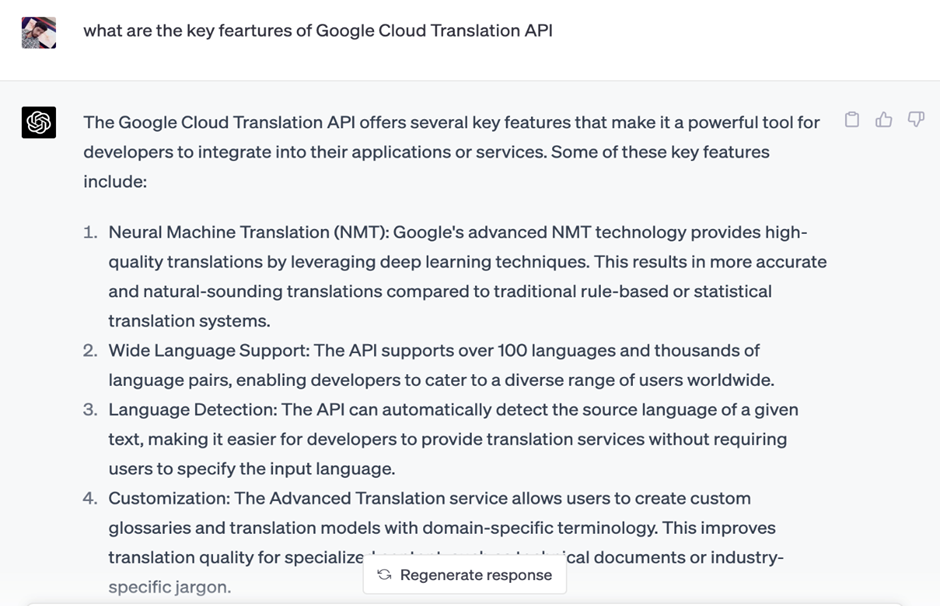
\includegraphics[width = 13.5cm]{Google Trans API.png}
    \caption{ChatGPT prompt and response to acquire more information about key features of Google Cloud Translation API}
    \label{fig:translationapi}
\end{figure}
\vspace{5pt}

As seen in \ref{fig:translationapi}, we utilized the ChatGPT tool in the modeling process to identify the key features of the Google Cloud Translation API.
\vspace{5pt}

\begin{figure}[hbtp]
    \centering
    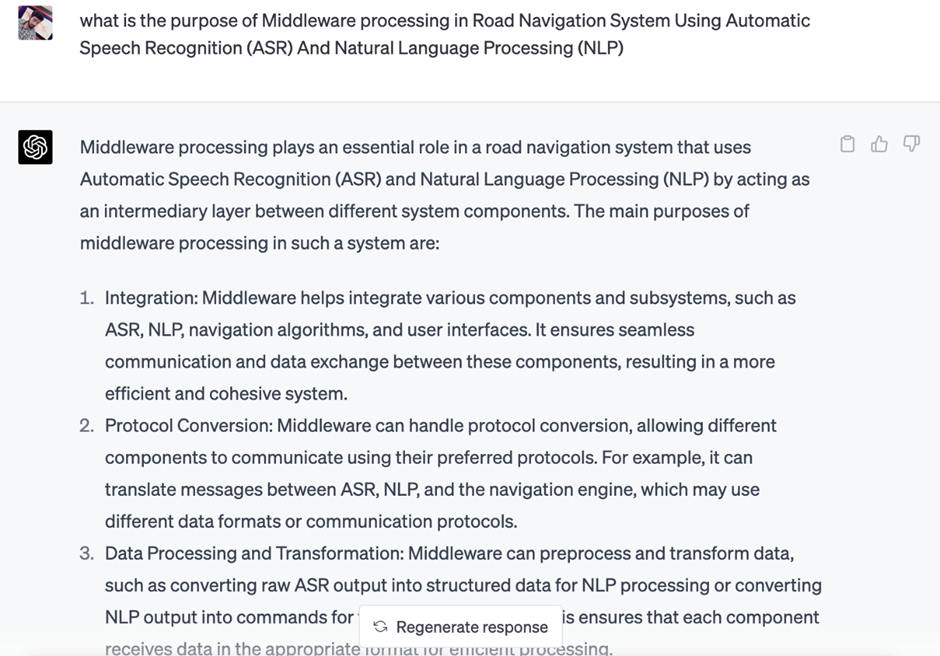
\includegraphics[width = 13.5cm]{Middleware.png}
    \caption{ChatGPT prompt and response to understand the role of middleware processing}
    \label{fig:middleware}
\end{figure}
\vspace{5pt}

As seen in \ref{fig:middleware}, we leveraged ChatGPT tool to help us understand the role and purpose of Middleware processing in our proposed system. 
\newpage

\begin{figure}[hbtp]
    \centering
    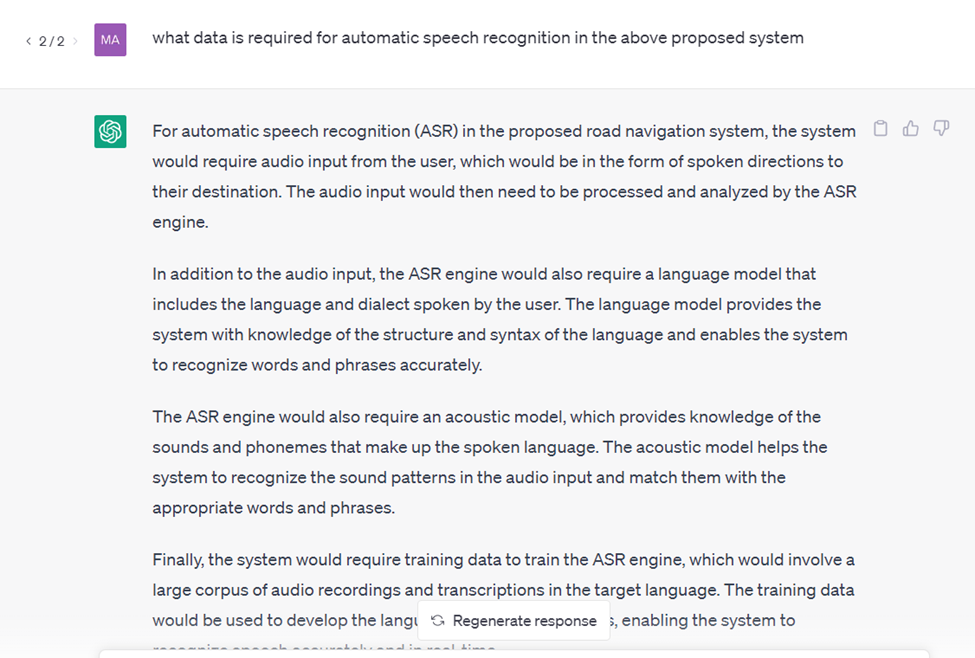
\includegraphics[width = 13.5cm]{ASR.png}
    \caption{ChatGPT prompt and response to acquire more information about data needed for ASR component}
    \label{fig:ASR}
\end{figure}


As seen in \ref{fig:ASR}, as part of our data understanding process, we turned to ChatGPT tool to help us identify the specific type of data that would be required for our Automatic Speech Recognition (ASR) component. 
\vspace{5pt}

\section{Grammarly} 
\vspace{5pt}

\begin{figure}[hbtp]
    \centering
    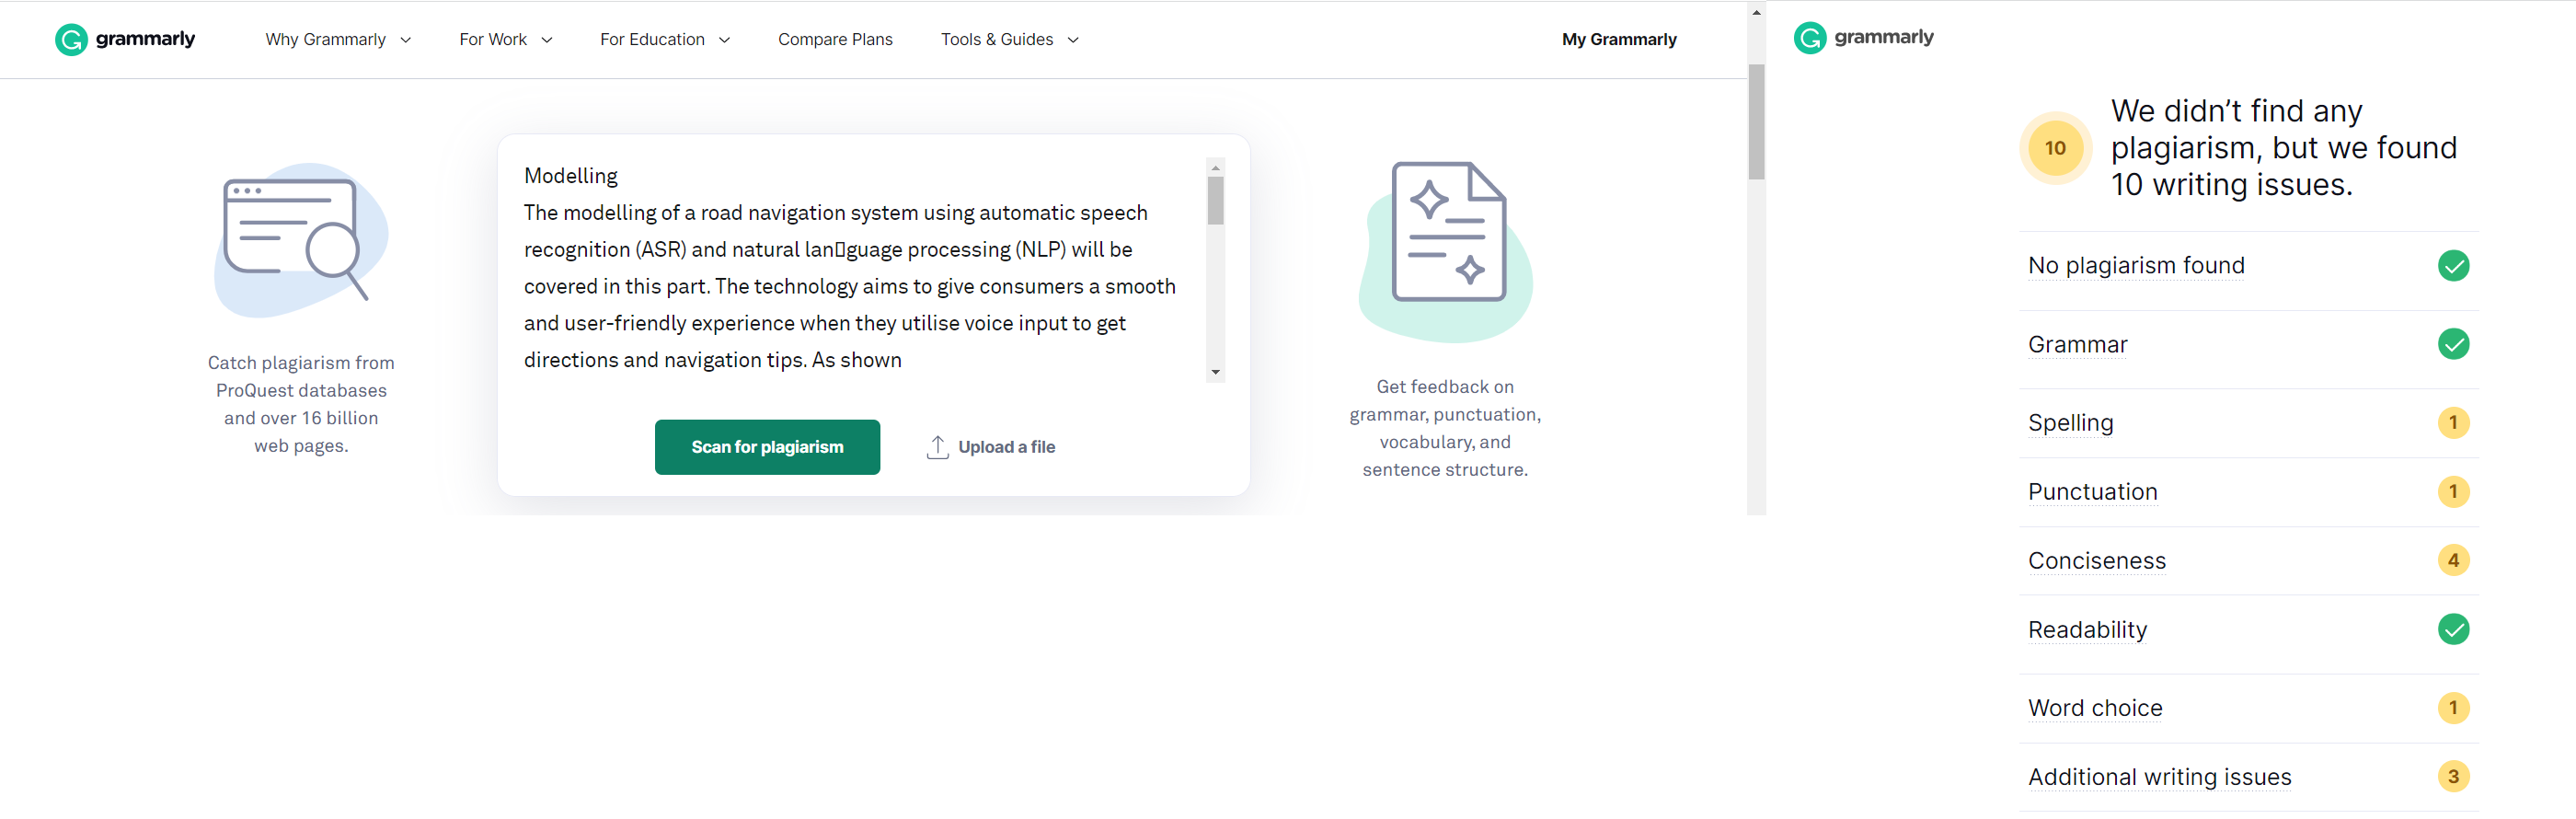
\includegraphics[width = 13.5cm]{Merged_document.png}
    \caption{Use of Grammarly for our proposal}
    \label{fig:Grammarly}
\end{figure}
\vspace{5pt}

As shown in \ref{fig:Grammarly}, we also utilized Grammarly, a comprehensive grammar checking tool, to enhance the language of our proposal and for checking grammar, spelling, punctuation, and style.
\vspace{5pt}

In conclusion, the combination of ChatGPT, Grammarly, and Google Scholar played a crucial role in the success of our research proposal. They helped us communicate our ideas in a clear, accurate, and professional manner.
\vspace{5pt}

\bibliographystyle{unsrt}
\bibliography{refs}

\end{document}
